\label{sec:overview}
\begin{figure}
	\centering
		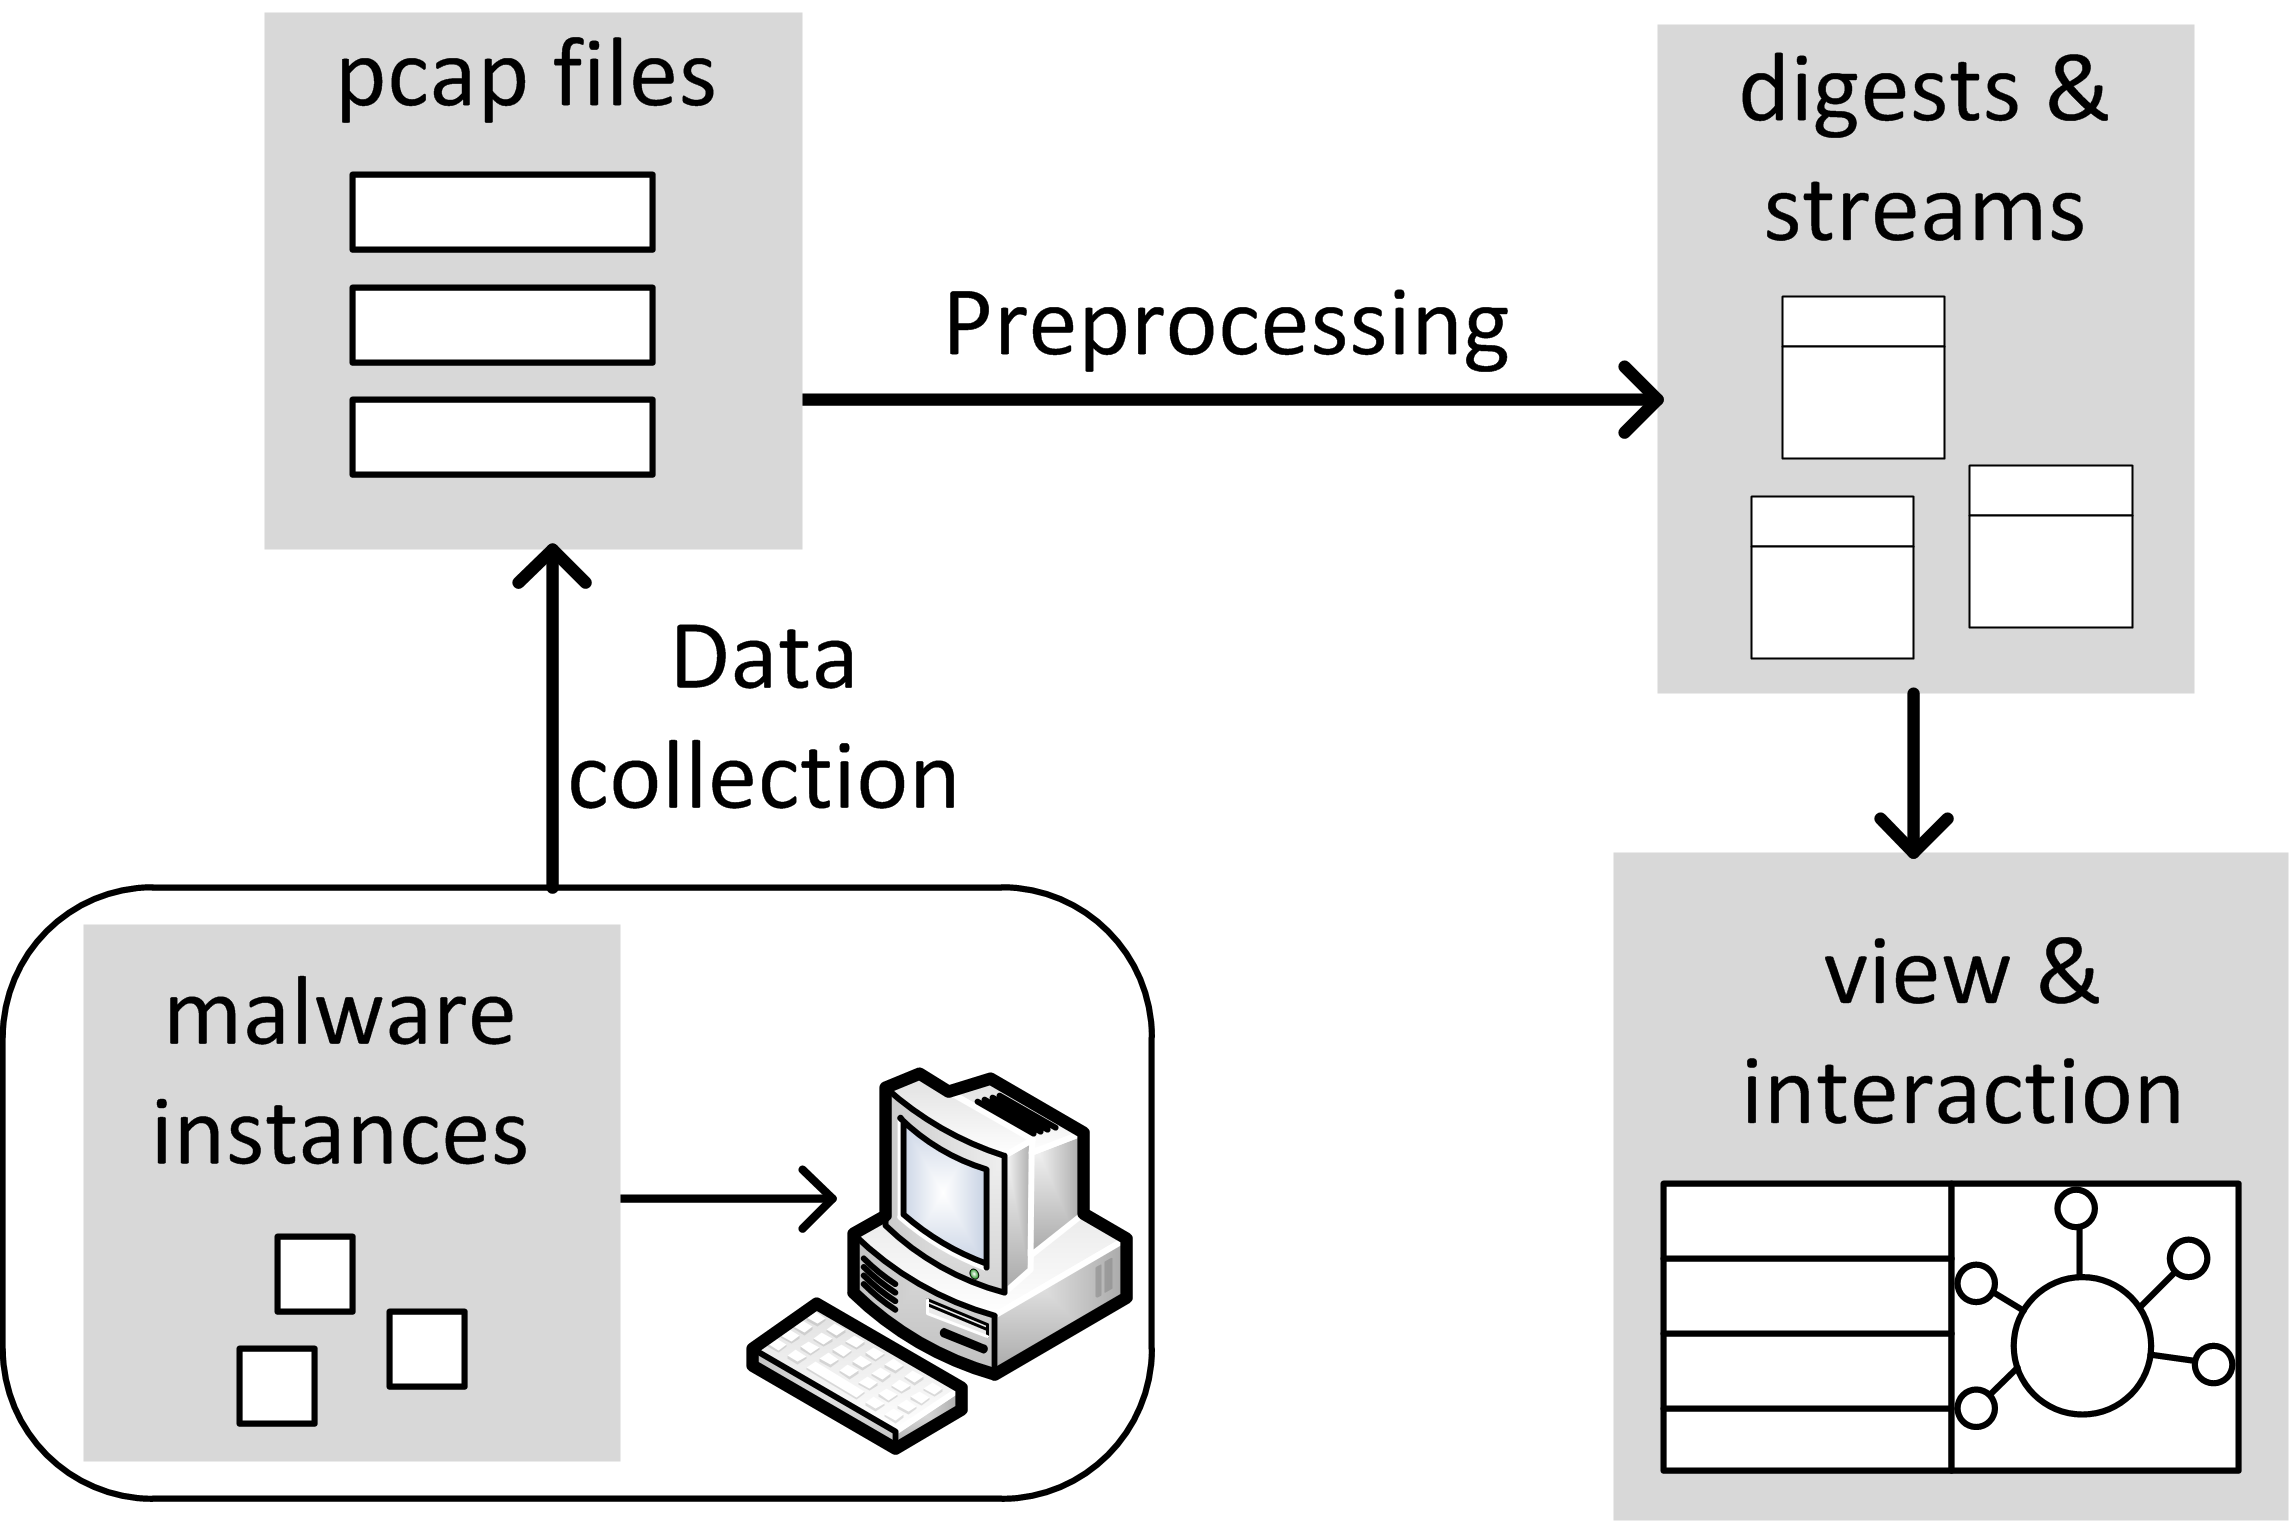
\includegraphics[width=\linewidth]{pics/Overview.png}
	\caption{The overview of our malware visual analytic system. The user-end view and interaction rely on three primary modules: data collection, preprocessing and visualization.}
		\label{fig:Overview}
\end{figure}

We show an overview of our malware visual analytic system in
Figure~\ref{fig:Overview}, and discuss how malware network data are captured,
processed and visualized in this section. This process consists of three
primary steps: \emph{data collection}, \emph{preprocessing}, and
\emph{visualization}.

\textbf{Data sources.} First, we gather a corpus of malware samples to use for
evaluation purposes. 200 MD5 unique malware samples were randomly selected from
malware collected during April 2011. We use multiple sources that provide
approximately 6,000 MD5 distinct samples per day taken from low interaction
honeypots, web crawlers, spam email filters, and user submissions. We restrict
our test set to only malware samples that exhibit network behavior during
execution. We analyze the malicious binaries by executing them for three minutes
in a virtualized dynamic malware analysis system that runs malware samples in
kvm~\cite{kvm} and records all the network traffic into packet traces as pcap
files\footnote{\url{http://www.tcpdump.org}}. Our visualization system is not
dependent on any particular dynamic analysis system and similar systems
described in the literature could serve as drop-in
replacements~(\cite{Bayer06}~\cite{Dinaburg08}),
Precautions were taken to prevent the executing malware from acting
maliciously; specifically, we redirect SMTP traffic to a spam trap, blocked
connections to ports commonly used by exploits and blocked traffic to other
local machines.

\textbf{Preprocessing.} Next, we parse pcap files into a set of appropriately
formatted documents which we refer to as malware entities. Each entity is of
the form

\verb+<Digest D | ArrayList<Stream> S>+

The structure \emph{Digest} consists of a sample's MD5, the total number of
packets, the total size of transmission, the total number of streams, and the
packet trace's duration. The list of streams are extracted from the protocol
information in the pcap file. Specifically, each stream includes attributes
such as host~(IP or domain name), protocol~(DNS or TCP), number of
packets~($n$), size of transmission~($z$), offset from the initial start
time~($s$), duration~($t$), and whether the stream ended successfully or not. A
DNS stream is defined as a DNS request and its corresponding response and a TCP
stream begins with a 3-way TCP handshake and concludes with successful or
unsuccessful termination.

\textbf{Visualization.} The visualization module generates table views and cell
views. Given a set of parsed and preprocessing entities, the user browses the
table of digests and selects one or more targets for analysis. Then, the
application generates a stream table and a cell view for each selected entity.
Our attributes mapping and layout algorithms run in real-time for most of the
malware entities supplied. In a typical visual analysis scenario, the user
interacts with the cell view by selecting a `cilium' that represents a stream of
interest. Details of the stream, such as its host IP and country code, are
displayed at the disk panel located at the center of the cell view. The user
can adjust the layout parameters for the circular timeline interactively so as
to improve the clarity of the set of cilia~(Sec.~\ref{sec:timeline}).

